%!TEX root = ../dokumentation.tex

\chapter{System Design}
\label{ch:design}

\section{Shared Data Layer}

Both the classical RAG pipeline and the agent-based system operate over an identical document corpus. This design decision is fundamental to the comparability of the evaluation: if either system were to ingest different content, differences in retrieval quality could not be attributed to architectural choices alone. The shared data layer therefore serves as the controlled variable in the experimental design, ensuring that all observed differences in latency, quality, and cost arise from the retrieval and generation strategies rather than from corpus coverage.

\subsection{Data Source Selection and Justification}

Enterprise knowledge environments are characterised by structural heterogeneity: relevant information is distributed across issue trackers, collaborative wikis, and document repositories, each imposing different constraints on document length, information density, and query semantics \cite{gao2023ragsurvey}. A retrieval system evaluated on documents drawn from a single structural type cannot demonstrate how it performs under this heterogeneity. Three structurally distinct source types are therefore used in this thesis, each selected to serve as a convincing open-source proxy for a category of enterprise documentation.

\textbf{GitHub Issues as a Jira proxy.} Issue tracker entries are short, metadata-rich documents with discrete structured fields—status, labels, assignees—alongside free-text description and comment threads. Closed issues from \texttt{kubernetes/kubernetes} and \texttt{microsoft/vscode} are used, providing 200 records after filtering for substantive body text (minimum 200 characters) and at least one comment. Closed issues are preferred because they contain resolution context alongside the original problem description, making them richer sources for question-answer pair generation. The Kubernetes repository provides canonical cloud-native infrastructure issues; the VS Code repository contributes developer-tooling issues, broadening topical coverage within the source type.

\textbf{Markdown and RST documentation as a Confluence proxy.} Collaborative wiki pages are discursive, medium-length documents organised by human-authored headings. Three repositories are cloned using sparse checkout to minimise bandwidth: \texttt{kubernetes/website} (English documentation subtree), \texttt{ansible/ansible-documentation} (RST format, infrastructure automation), and \texttt{cncf/tag-observability} (full clone; includes the 68\,KB observability whitepaper and working-group documents). After markup stripping and minimum-length filtering, 1\,283 documents are retained.

\textbf{PDF whitepapers as a SharePoint proxy.} Formal document repositories typically contain long, hierarchically structured texts—policy documents, technical reports, architectural specifications. Thirteen CNCF whitepapers and strategy documents are downloaded from the \texttt{cncf/tag-security}, \texttt{cncf/tag-storage}, \texttt{cncf/tag-app-delivery}, \texttt{cncf/foundation}, and \texttt{cncf/wg-serverless} repositories, yielding 140 extractable sections after discarding graphics-only pages.

\textbf{Thematic coherence.} All three source types are drawn from the cloud-native and Kubernetes ecosystem. This choice is deliberate: shared topical coverage across source types makes cross-document synthesis queries genuinely answerable — a question about Kubernetes security can in principle be addressed by an issue, a documentation page, and a CNCF whitepaper simultaneously. Without thematic overlap, multi-source synthesis queries would be unanswerable by design, removing one of the most important dimensions of the evaluation. Table~\ref{tab:corpus} summarises the resulting corpus.

\begin{table}[ht]
\centering
\small
\setlength{\tabcolsep}{4pt}
\caption{Corpus statistics after acquisition and filtering.}
\label{tab:corpus}
\begin{tabular}{p{5.0cm}p{3.5cm}rr}
\hline
\textbf{Source type} & \textbf{Enterprise proxy} & \textbf{Records} & \textbf{Avg.\ words} \\
\hline
GitHub Issues & Jira tickets & 200 & 2\,434 \\
Markdown / RST documentation & Confluence wiki & 1\,283 & 646 \\
PDF whitepaper sections & SharePoint documents & 140 & 952 \\
\hline
\textbf{Total} & & \textbf{1\,623} & \\
\hline
\end{tabular}
\end{table}

\subsection{Unified Document Schema}

Every record produced by the acquisition pipeline is normalised to a shared JSON schema before it is consumed by either system. Normalisation serves two purposes: it decouples source-specific acquisition logic from the retrieval systems, and it ensures that both the RAG pipeline and the agent-based system receive identically structured inputs, making downstream comparisons valid.

Each record contains five top-level fields. The \texttt{source\_type} field carries one of three fixed values—\texttt{github\_issue}, \texttt{markdown\_doc}, or \texttt{pdf\_whitepaper}—and is used by the agent's routing logic to identify which retrieval tool to invoke. The \texttt{id} field is a globally unique string constructed from the source repository and a document-specific identifier (issue number, file path relative to the repository root, or document name plus section index). The \texttt{title} field contains the issue title, the first heading extracted from the document, or the leading text of the first non-junk page of the PDF section. The \texttt{content} field contains plain text, stripped of all markup, capped at 8\,000 characters to keep token counts manageable during embedding and generation. The \texttt{metadata} object carries source-specific fields used for provenance tracing and, in the case of GitHub Issues, for label-based analysis.

\begin{table}[ht]
\centering
\small
\setlength{\tabcolsep}{4pt}
\caption{Unified document schema shared by both retrieval systems.}
\label{tab:schema}
\begin{tabular}{p{4.6cm}p{1.3cm}p{7.7cm}}
\hline
\textbf{Field} & \textbf{Type} & \textbf{Description} \\
\hline
\texttt{source\_type}         & string  & \texttt{github\_issue} $|$ \texttt{markdown\_doc} $|$ \texttt{pdf\_whitepaper} \\
\texttt{id}                   & string  & Globally unique document identifier \\
\texttt{title}                & string  & Document or section heading \\
\texttt{content}              & string  & Plain-text body, max 8\,000 characters \\
\texttt{metadata.repo}        & string  & Source repository or document name \\
\texttt{metadata.url}         & string  & Canonical URL of the source \\
\texttt{metadata.labels}      & array   & Issue labels; empty for docs and PDFs \\
\texttt{metadata.created\_at} & string  & ISO\,8601 timestamp or publication date \\
\hline
\end{tabular}
\end{table}

The three source types produce separate JSONL files — \texttt{github\_issues.jsonl}, \texttt{markdown\_docs.jsonl}, and \texttt{pdf\_whitepapers.jsonl} — which are read independently by the ingestion components of both systems. The separation by source type is intentional: it allows each system to construct source-specific indexes or tool backends without requiring a schema change, while the shared field names ensure that logging, evaluation, and post-hoc analysis code operates identically across all three.

\subsection{Ingestion Data Flow}

Acquisition and normalisation proceed in three parallel pipelines, one per source type, before converging at the JSONL files that feed both retrieval systems. Figure~\ref{fig:dataflow} illustrates the overall flow.

\begin{figure}[ht]
  \centering
  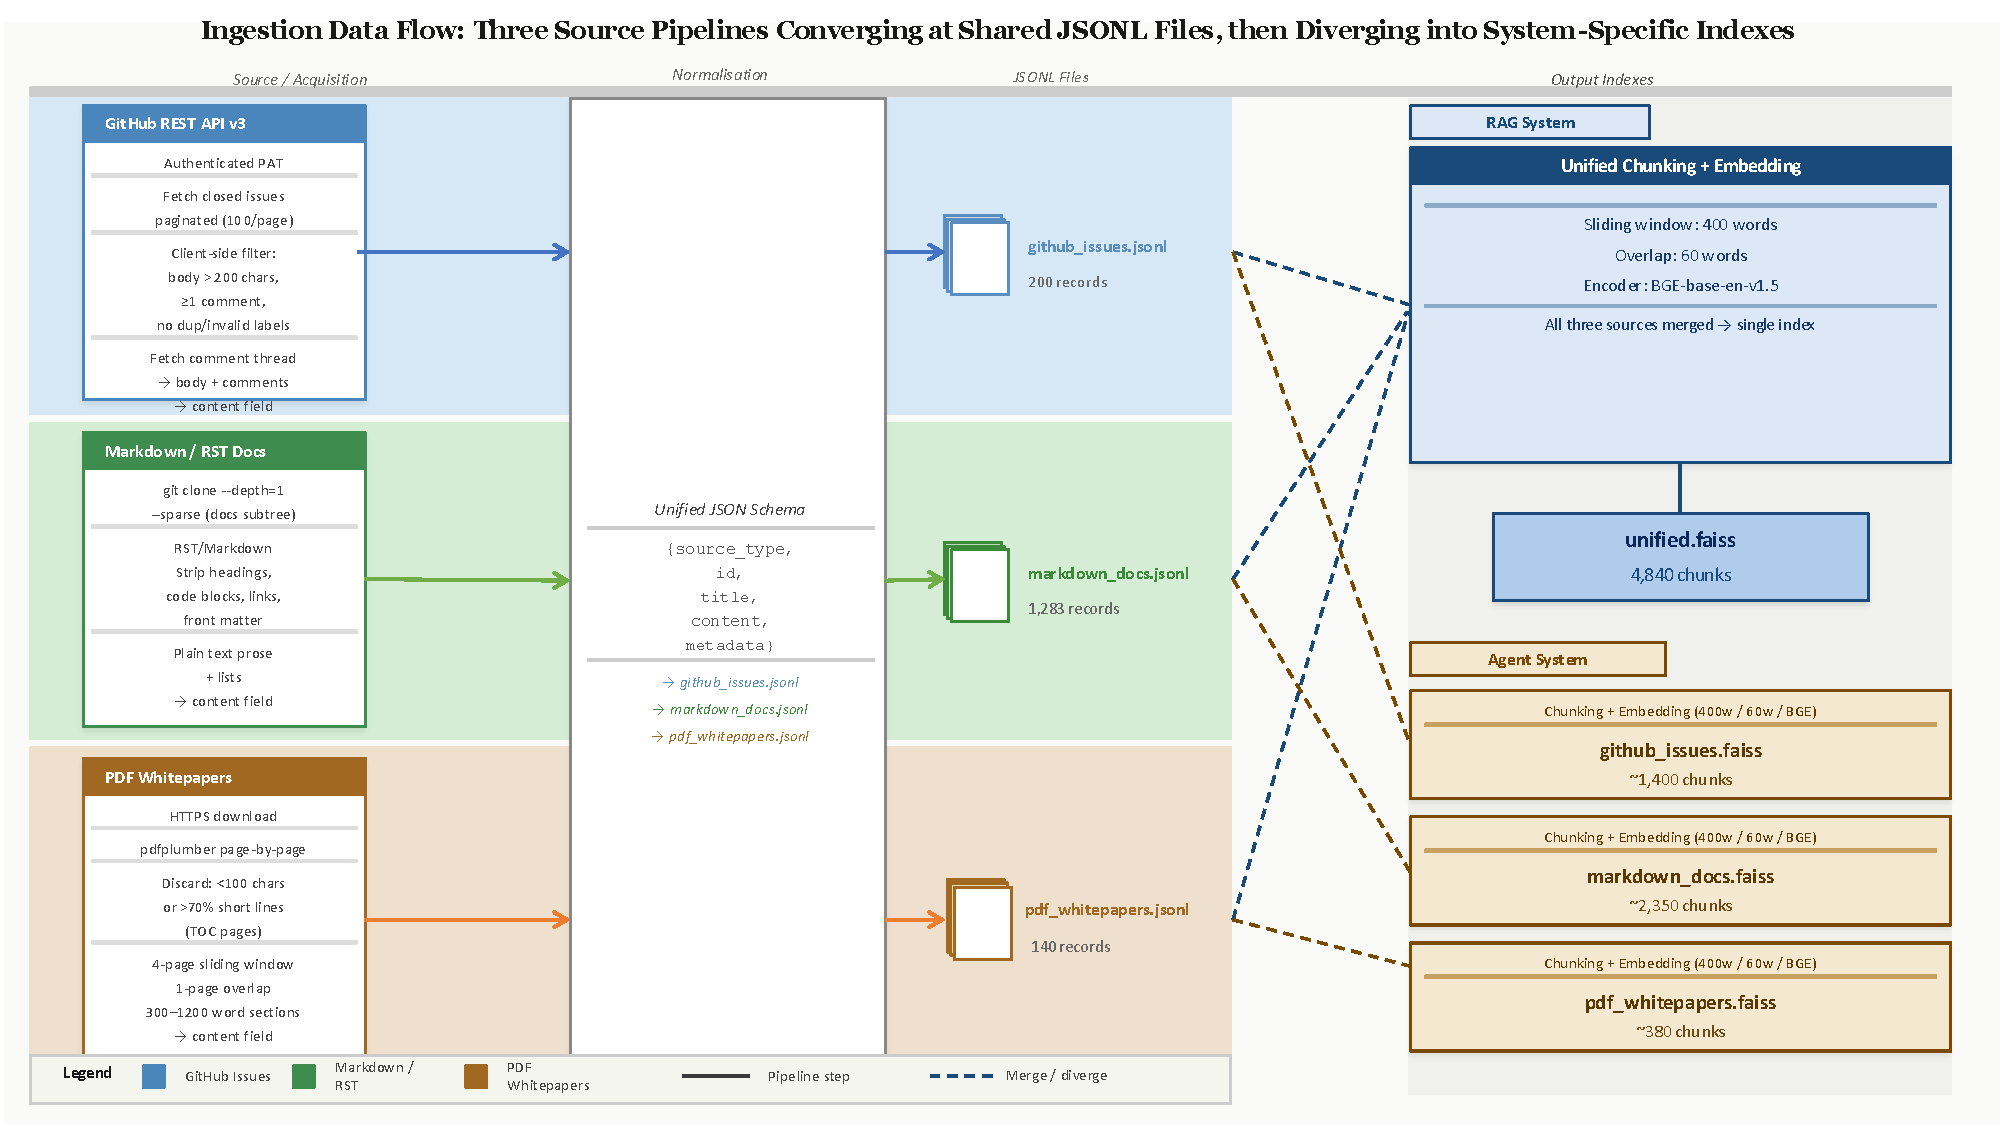
\includegraphics[width=\linewidth]{images/ingestion_flow}
  \caption{Ingestion data flow: three source pipelines converging at shared JSONL files, then diverging into system-specific indexes. Chunking parameters (400-word sliding window, 60-word overlap) and the BGE-base-en-v1.5 embedding model are shared across both systems; the sole architectural difference is a single unified index for RAG versus three per-source indexes for the agent.}
  \label{fig:dataflow}
\end{figure}

\textbf{GitHub Issues.} The GitHub REST API v3 is queried with an authenticated Personal Access Token, raising the rate limit from 60 to 5\,000 requests per hour. Closed issues are fetched in pages of 100, filtered client-side against the criteria defined in Section~\ref{ch:data}, and their comment threads are fetched in a subsequent request per issue. The body and comments are concatenated with a separator and written as a single \texttt{content} field.

\textbf{Markdown and RST documentation.} Repositories are cloned with \texttt{git clone \texttt{-{}-}depth=1 \texttt{-{}-}filter=blob:none \texttt{-{}-}sparse}, populating only the documentation subtree. This minimises bandwidth and avoids downloading build artefacts, themes, and binary assets. RST files from the Ansible documentation are processed identically to Markdown files; both formats are reduced to plain text by a regular-expression pipeline that strips headings, fenced code blocks, hyperlinks, shortcodes, and front matter, preserving only the readable prose and list content.

\textbf{PDF whitepapers.} PDFs are downloaded via authenticated HTTPS and processed with \texttt{pdfplumber}. Text is extracted page by page; pages with fewer than 100 characters of extracted text or exhibiting a table-of-contents structure (more than 70\,\% of lines shorter than 50 characters) are discarded. The remaining pages are grouped into overlapping four-page windows with a one-page overlap, producing sections of 300–1\,200 words that are large enough to contain coherent argumentation yet small enough to fit within a typical retrieval context window.

At the convergence point, both retrieval systems read from the same three JSONL files. The RAG pipeline passes all records through a single unified chunking and embedding stage, producing one vector index. The agent-based system ingests each JSONL file into a separate source-specific index, one per tool. This architectural divergence is one of the key design differences examined in the evaluation.

\section{Classical RAG Pipeline Architecture}

The classical RAG pipeline transforms raw corpus documents into a queryable knowledge store and, at query time, retrieves and synthesises the most relevant passages into a grounded answer. The implementation comprises eight discrete steps organised into two phases: an offline ingestion phase that runs once against the full corpus, and an online query phase that executes on every user request.

\subsection{Pipeline Stages}

Ingestion proceeds sequentially through four steps. Documents are loaded from the three source JSONL files, split into overlapping fixed-size chunks, encoded into dense vector representations by the embedding model, and added to a persistent FAISS index. At the end of ingestion, 1,623 corpus records have been expanded into 4,840 chunks, each carrying its parent document's source type, title, and metadata. The FAISS index and the chunk metadata store are written to disk and reloaded on startup, so the computationally intensive embedding step is never repeated unless the corpus changes.

The online query phase executes four further steps for each incoming question. The query is encoded by the same embedding model and the resulting vector is compared against all indexed chunk vectors to retrieve the twenty closest candidates. A cross-encoder reranker then scores each candidate against the query and returns the five highest-scoring chunks. These chunks are assembled into a numbered context block and passed to the language model alongside a system prompt that instructs the model to answer using only the supplied passages. Latency and token counts are captured for every query and appended to a structured JSONL log, producing the measurement records used in Chapter~\ref{ch:results}.

\subsection{Chunking Strategy}

Each corpus document is split into overlapping windows of 400 words with a 60-word overlap between consecutive windows. The step size between window starts is therefore 340 words, meaning that the first 60 words of each chunk also appear at the end of the preceding chunk. This overlap preserves semantic continuity across boundaries: a sentence or argument that spans a chunk boundary is fully represented in at least one chunk, ensuring that a relevant passage is not fragmented out of the index \cite{gao2023ragsurvey}.

Chunking operates on whitespace-delimited word lists rather than on subword tokens produced by a transformer tokeniser. This makes the chunking step independent of any specific model vocabulary, so that the embedding or reranker model can be replaced without recalibrating chunk sizes. In practice, a 400-word chunk corresponds to approximately 480–550 subword tokens for English technical prose, which falls within the 512-token context limit of the embedding model and well below the 8,192-token limit of the cross-encoder.

The 400-word target balances retrieval precision against contextual coherence, a trade-off documented explicitly in the Advanced RAG literature \cite{gao2023ragsurvey}. Shorter chunks increase the likelihood that a retrieved passage is topically homogeneous, but risk fragmenting multi-step arguments that require surrounding context to be interpretable; longer chunks preserve coherence but dilute the relevance signal. The 60-word overlap and 400-word window together place this implementation within the Advanced RAG category of the Naive / Advanced / Modular taxonomy, distinguishing it from Naive RAG pipelines that apply fixed splits without overlap.

\subsection{Embedding Model and Vector Store}

Chunks and queries are encoded using \texttt{BAAI/bge-base-en-v1.5}, a 768-dimensional bi-encoder model executed locally via the \texttt{sentence-transformers} library. The model was selected from the MTEB Retrieval leaderboard as a top-performing open-weight model at its parameter scale, requiring no external API call and incurring no per-token cost. BGE models are trained with an asymmetric query--document encoding scheme: at query time, the string \textit{``Represent this sentence for searching relevant passages:''} is prepended to the raw query before encoding, while document chunks are encoded without any prefix. This asymmetry is required for the model to produce embeddings that align query intent with document content; omitting the prefix at query time measurably degrades retrieval quality \cite{gao2023ragsurvey}.

All embeddings are L2-normalised to unit length before any similarity computation, both at ingestion time and at query time. Normalisation allows the FAISS \texttt{IndexFlatIP} index to compute cosine similarity via the inner product: for unit-length vectors $\mathbf{u}$ and $\mathbf{v}$, the relation $\mathbf{u} \cdot \mathbf{v} = \cos\theta$ holds, making inner-product maximisation equivalent to cosine similarity maximisation. Cosine similarity is preferred over raw inner product because it is magnitude-invariant — a longer chunk does not receive a spuriously high score simply by virtue of producing a larger embedding vector.

FAISS \texttt{IndexFlatIP} performs exact nearest-neighbour search over the full index without quantisation or approximation. At 4,840 vectors of dimension 768 stored as 32-bit floats, the index occupies approximately 14\,MB of memory and returns query results in under one second on the development hardware. Exact search is therefore practical at this corpus scale and avoids the recall penalty introduced by approximate methods such as HNSW or IVF clustering, which trade retrieval accuracy for speed at larger scales \cite{lewis2020rag}.

\subsection{Retrieval and Reranking}

Retrieval proceeds in two stages to exploit the complementary properties of bi-encoders and cross-encoders. In the first stage, the FAISS index returns the twenty document chunks whose embeddings have the highest cosine similarity to the embedded query. These twenty candidates are then passed to \texttt{cross-encoder/ms-marco-MiniLM-L-6-v2}, a cross-encoder model fine-tuned on the MS MARCO passage-ranking benchmark, which scores each query--chunk pair jointly by processing the concatenated pair as a single transformer input.

The key distinction between the two stages lies in how query and document representations are produced. Bi-encoders encode queries and documents independently and compare them post hoc; this enables sub-second retrieval over arbitrarily large indexes but prevents the model from attending to fine-grained token-level interactions between the two texts. Cross-encoders process both texts as a single input, allowing full cross-attention across the query--chunk boundary and producing substantially more accurate relevance scores at the cost of one forward pass per candidate \cite{gao2023ragsurvey}. Applying the cross-encoder only to the twenty FAISS candidates bounds its computational cost to a fixed and small number of inference calls regardless of index size, keeping online latency predictable.

The five highest-scoring chunks after reranking are passed to the generator. Each chunk carries both its FAISS cosine similarity score and its cross-encoder rerank score in the log record, providing a complete provenance trail for post-hoc analysis of retrieval behaviour. Temperature is set to zero for all generation calls to ensure fully deterministic outputs across evaluation runs, a requirement for the reproducibility of the evaluation described in Chapter~\ref{ch:data}. Two retrieval enhancements extend this baseline. Both were incorporated as a post-evaluation revision to the pipeline; the initial results that motivated their addition are presented in Chapter~\ref{ch:results}, and their implementation is detailed in Section~\ref{sec:rag-impl}.

\textbf{Hypothetical Document Embedding (HyDE)} addresses the semantic mismatch between query register and document register that constrains bi-encoder retrieval \cite{gao2023hyde}. Before querying the FAISS index, the language model generates a short hypothetical passage — two to three sentences — that directly answers the query. This passage is embedded without the BGE retrieval prefix, placing its vector in the same distributional region as stored document chunks rather than in the query subspace. The hypothesis vector replaces the query vector as the FAISS search input; the original query is preserved and used unchanged for cross-encoder reranking, so relevance scoring remains grounded in the actual question rather than in the generated passage.

\textbf{Maximal Marginal Relevance (MMR)} addresses the tendency of nearest-neighbour retrieval to return near-duplicate passages from the same document section \cite{carbonell1998mmr}. After the cross-encoder sorts the twenty candidates by relevance, MMR iteratively selects the five final passages by maximising a linear combination of relevance and diversity: at each step it picks the candidate that best balances a high normalised rerank score against low cosine similarity to the passages already selected. A relevance weight of $\lambda = 0.7$ gives relevance priority over diversity, ensuring the final context window is both topically focused and non-redundant. Figure~\ref{fig:rag_pipeline} illustrates the complete query-phase pipeline including both extensions.

\begin{figure}[ht]
  \centering
  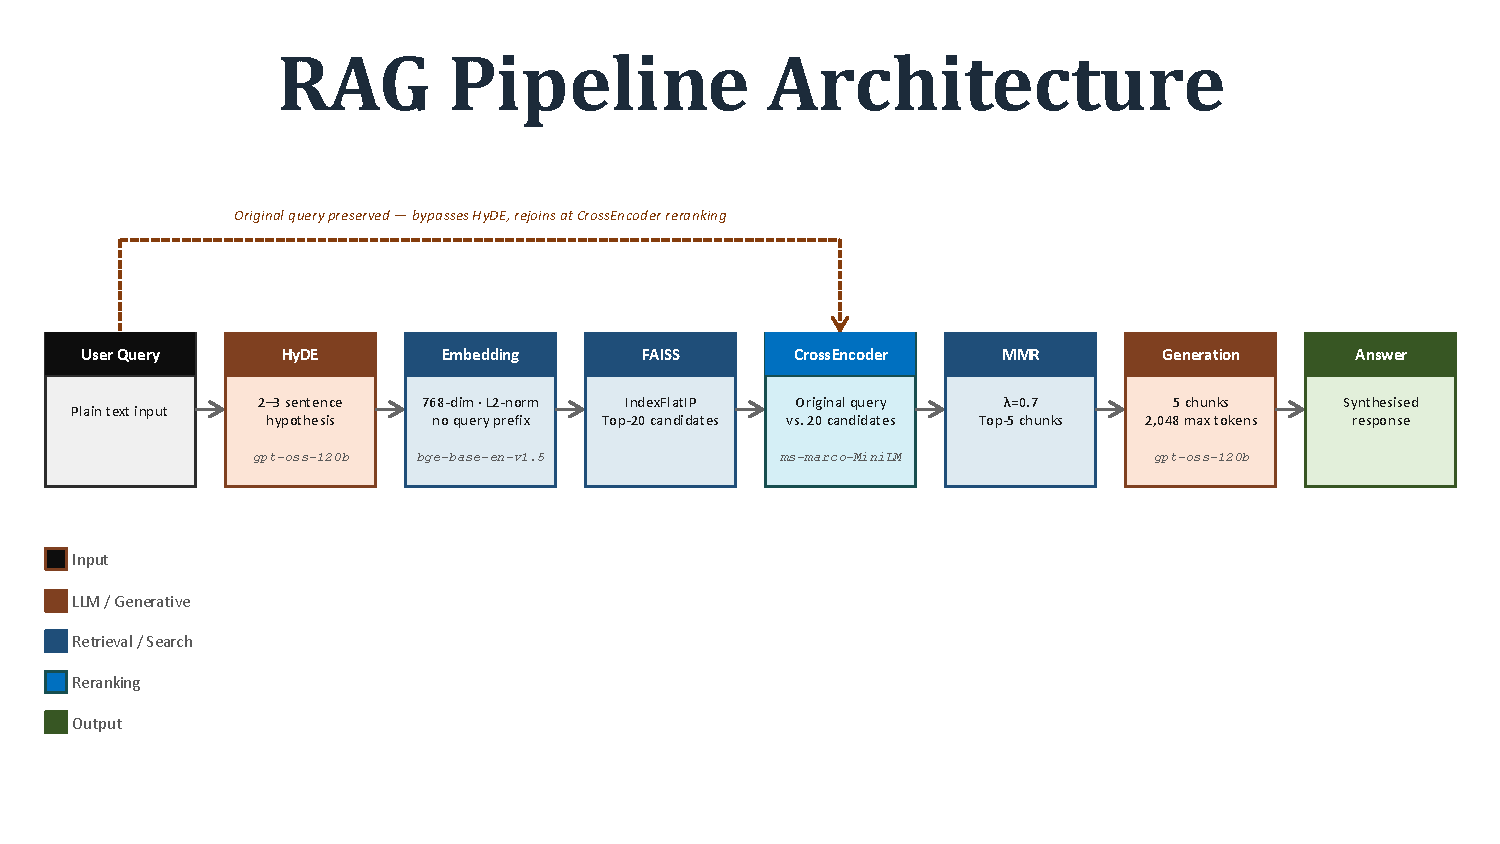
\includegraphics[width=\linewidth]{images/rag_pipeline}
  \caption{RAG pipeline query phase. The original query is passed to the LLM to generate a hypothetical passage (HyDE), whose embedding is used as the FAISS search vector. The original query is preserved for cross-encoder reranking, ensuring relevance scoring remains grounded in the actual question. MMR diversification ($\lambda = 0.7$) then selects the final five passages from the reranked pool before synthesis.}
  \label{fig:rag_pipeline}
\end{figure}

\section{Agent-Based System Architecture}

The agent-based system replaces the RAG pipeline's fixed retrieve-then-generate sequence with an iterative reasoning loop in which the language model selects and invokes retrieval tools based on the content and requirements of each query. Rather than encoding the entire corpus into a single unified index, the system exposes three source-specific retrieval tools and delegates the decision of which tool to call, in what order, and with what query formulation to the language model at runtime. The implementation follows the ReAct framework \cite{yao2023react} and is built using LangChain's agent scaffolding on top of the same language model endpoint and embedding infrastructure used by the RAG pipeline.

\subsection{The Agent Loop}

ReAct defines an interleaved reasoning and acting pattern in which a language model alternates between generating a \textit{Thought}—an explicit natural-language reasoning step—and taking an \textit{Action}—a structured tool call with explicit inputs \cite{yao2023react}. After each action, the tool's return value is appended to the context as an \textit{Observation}, and the model continues reasoning from the updated context until it emits a final answer prefixed with the token \textit{Final Answer}. This cycle constitutes a closed-loop process: unlike the single retrieval pass of the RAG pipeline, the agent can inspect retrieved evidence, judge its sufficiency, and issue further tool calls or reformulated queries before committing to a response.

The implementation uses LangChain's \texttt{create\_react\_agent} function, which binds the language model, the registered tool set, and a ReAct-format prompt into an executable agent definition, and \texttt{AgentExecutor}, which drives the reasoning cycle at runtime. The language model is accessed through LangChain's \texttt{ChatOpenAI} wrapper pointed at the same OpenAI-compatible endpoint used by the RAG pipeline—Ollama in development, AI Refinery during evaluation—with identical model identifier and temperature settings. A maximum iteration count of fifteen is enforced by the \texttt{AgentExecutor}; this bound accommodates queries that require all three tools in sequence while preventing unbounded loop growth on ambiguous or unanswerable inputs.

\subsection{Tools and Source Routing}

Three retrieval tools are registered with the agent, one per corpus source type. Each tool wraps a dedicated FAISS index constructed from the same corpus using the same 400-word sliding-window chunking, 60-word overlap, and BGE-base-en-v1.5 embedding model as the RAG pipeline. Separate per-source indexes are used rather than the RAG pipeline's unified index to reflect the architectural reality of enterprise knowledge environments, in which issue trackers, documentation platforms, and document repositories are independent systems with distinct search interfaces \cite{ferrazzi2026agenticrag}. An agent operating over a unified index would have no structural basis on which to make source-routing decisions; partitioning the indexes makes routing a genuine runtime choice with observable consequences for retrieval quality and, consequently, answer faithfulness.

\begin{table}[ht]
\centering
\small
\setlength{\tabcolsep}{4pt}
\caption{Agent retrieval tools and their source-type scope.}
\label{tab:agent_tools}
\begin{tabular}{lll}
\hline
\textbf{Tool name} & \textbf{Source type} & \textbf{Enterprise proxy} \\
\hline
\texttt{search\_github\_issues}   & GitHub Issues     & Jira tickets \\
\texttt{search\_markdown\_docs}   & Markdown/RST docs & Confluence wiki \\
\texttt{search\_pdf\_whitepapers} & CNCF PDF sections & SharePoint documents \\
\hline
\end{tabular}
\end{table}

Each tool applies the same two-stage retrieval used in the RAG pipeline: twenty nearest-neighbour candidates are retrieved from the tool's FAISS index and then reranked by \texttt{cross-encoder/ms-marco-MiniLM-L-6-v2} to a top-five result set. This ensures that retrieval quality per tool call is directly comparable to the RAG pipeline's retrieval quality, so that any differences in final answer quality reflect the agent's routing and synthesis behaviour rather than differences in the underlying retrieval mechanics.

\subsection{Orchestration Logic}

Source routing is implemented entirely through the natural-language descriptions attached to each tool in the ReAct system prompt. No explicit rule-based dispatch logic is implemented; the language model reads each tool's description and selects the appropriate tool based on query semantics at each reasoning step. The descriptions are written to reflect the structural characteristics and dominant query patterns of each source type: the GitHub Issues tool is described as appropriate for bug reports, error messages, and issue resolutions; the documentation tool for conceptual explanations, how-to guides, and configuration references; the whitepaper tool for standards, best practice recommendations, and maturity frameworks. This design is authentic to the ReAct pattern, in which tool selection is part of the Thought generation step \cite{yao2023react}, and avoids brittle keyword-based dispatch that would require maintenance whenever the corpus is extended.

Tool observations are returned as formatted plain text containing the five reranked chunks, each prefixed with its source type, document title, and cosine similarity score. This format supplies the language model with the provenance information required to attribute claims and to judge whether a further tool call is warranted, while keeping each observation compact enough to avoid exhausting the context window across multi-step queries. The agent may call the same tool more than once with a reformulated query if the first observation is insufficient, or it may call multiple tools in sequence for cross-source synthesis queries.

All tool calls, their inputs, and their observations are recorded in a structured \texttt{agent\_trace} field appended to each log record alongside the query, final answer, total latency, and token counts. The log schema is a strict superset of the RAG pipeline's schema: all shared fields—query, answer, latency, token counts, and retrieved chunks—are produced identically by both systems, while the \texttt{agent\_trace}, tool-call count, and source-routing fields are present only in agent logs. This shared outer schema ensures that the evaluation infrastructure processes both systems' outputs without modification. Figure~\ref{fig:single_agent} illustrates the complete single-agent loop.

\begin{figure}[ht]
  \centering
  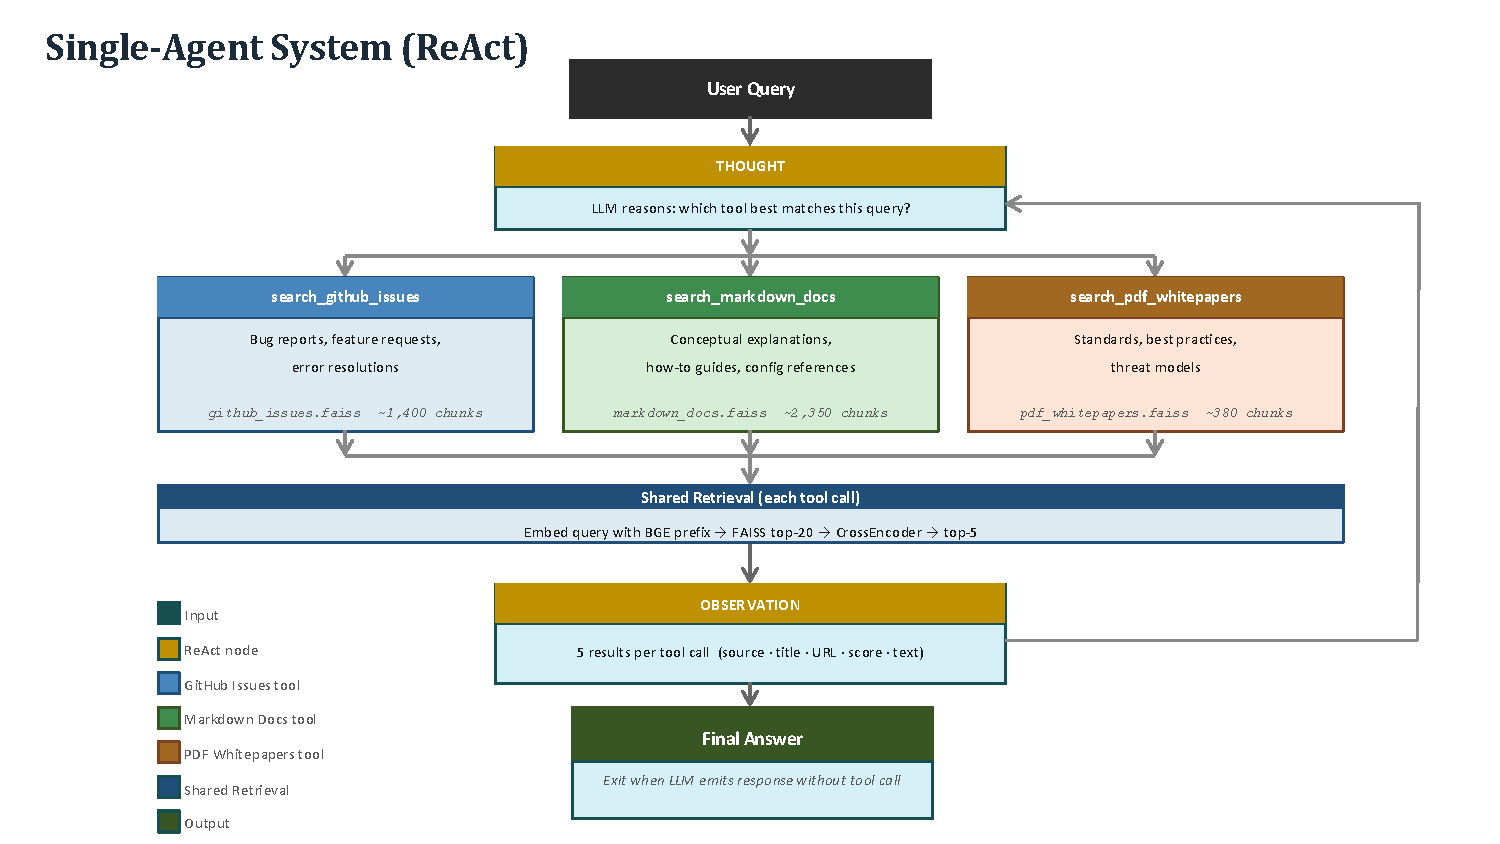
\includegraphics[width=\linewidth]{images/single_agent}
  \caption{Single-agent ReAct loop. The language model alternates between Thought (reasoning) and Action (tool call) steps; each tool observation is appended to the growing context window and the cycle repeats until the model emits a final answer without a tool call, or the 15-iteration ceiling is reached.}
  \label{fig:single_agent}
\end{figure}

\subsection{Multi-Agent Coordination Architecture}
\label{subsec:multi-agent-design}

The multi-agent architecture was designed as a corrective response to structural failure modes identified during single-agent evaluation: context accumulation across the ReAct loop exhausted the iteration ceiling, causing 41~per cent of queries to fail before a final answer was produced. Rather than lengthening the iteration limit further, the architecture eliminates the loop entirely.

\begin{sloppypar}
The design is a two-node LangGraph \texttt{StateGraph}. The first node, \texttt{retrieve\_all\_sources}, queries all three source-specific FAISS indexes sequentially — GitHub Issues, Markdown documentation, and PDF whitepapers — applying the same cross-encoder reranking pipeline used in both the RAG and single-agent systems to each source in turn, and accumulating at most fifteen chunks in total, five per source. The second node, \texttt{synthesize}, receives the pooled passages as a single bounded context window and issues exactly one language model call to produce the final answer. No further retrieval is possible once synthesis begins; the context presented to the model is fixed at the point the first node completes.
\end{sloppypar}

Three design properties distinguish this architecture from the single-agent system. There is no reasoning loop and therefore no iteration limit and no risk of\linebreak[0] \texttt{GraphRecursionError}. The context window per query is fixed at fifteen chunks regardless of query type or complexity, making the per-query token budget fully predictable. All three sources are queried on every request, so source coverage is an architectural guarantee rather than a model-driven decision \cite{xi2023rise}. These properties come at a cost: the multi-agent system cannot direct retrieval effort selectively toward the most relevant source, nor can it reformulate a query after inspecting an initial observation.

The multi-agent reuses the per-source FAISS indexes constructed by \texttt{agent/ingest.py} and the \texttt{SourceRetriever} class from \texttt{agent/tools.py}, adding no new ingestion infrastructure. The primary trade-off relative to the single agent is coverage guarantee versus query-adaptive selectivity: the multi-agent provides complete source coverage at the cost of the ability to concentrate retrieval on a single source for queries whose answer is localised to one part of the corpus. Figure~\ref{fig:multi_agent} illustrates the architecture.

\begin{figure}[ht]
  \centering
  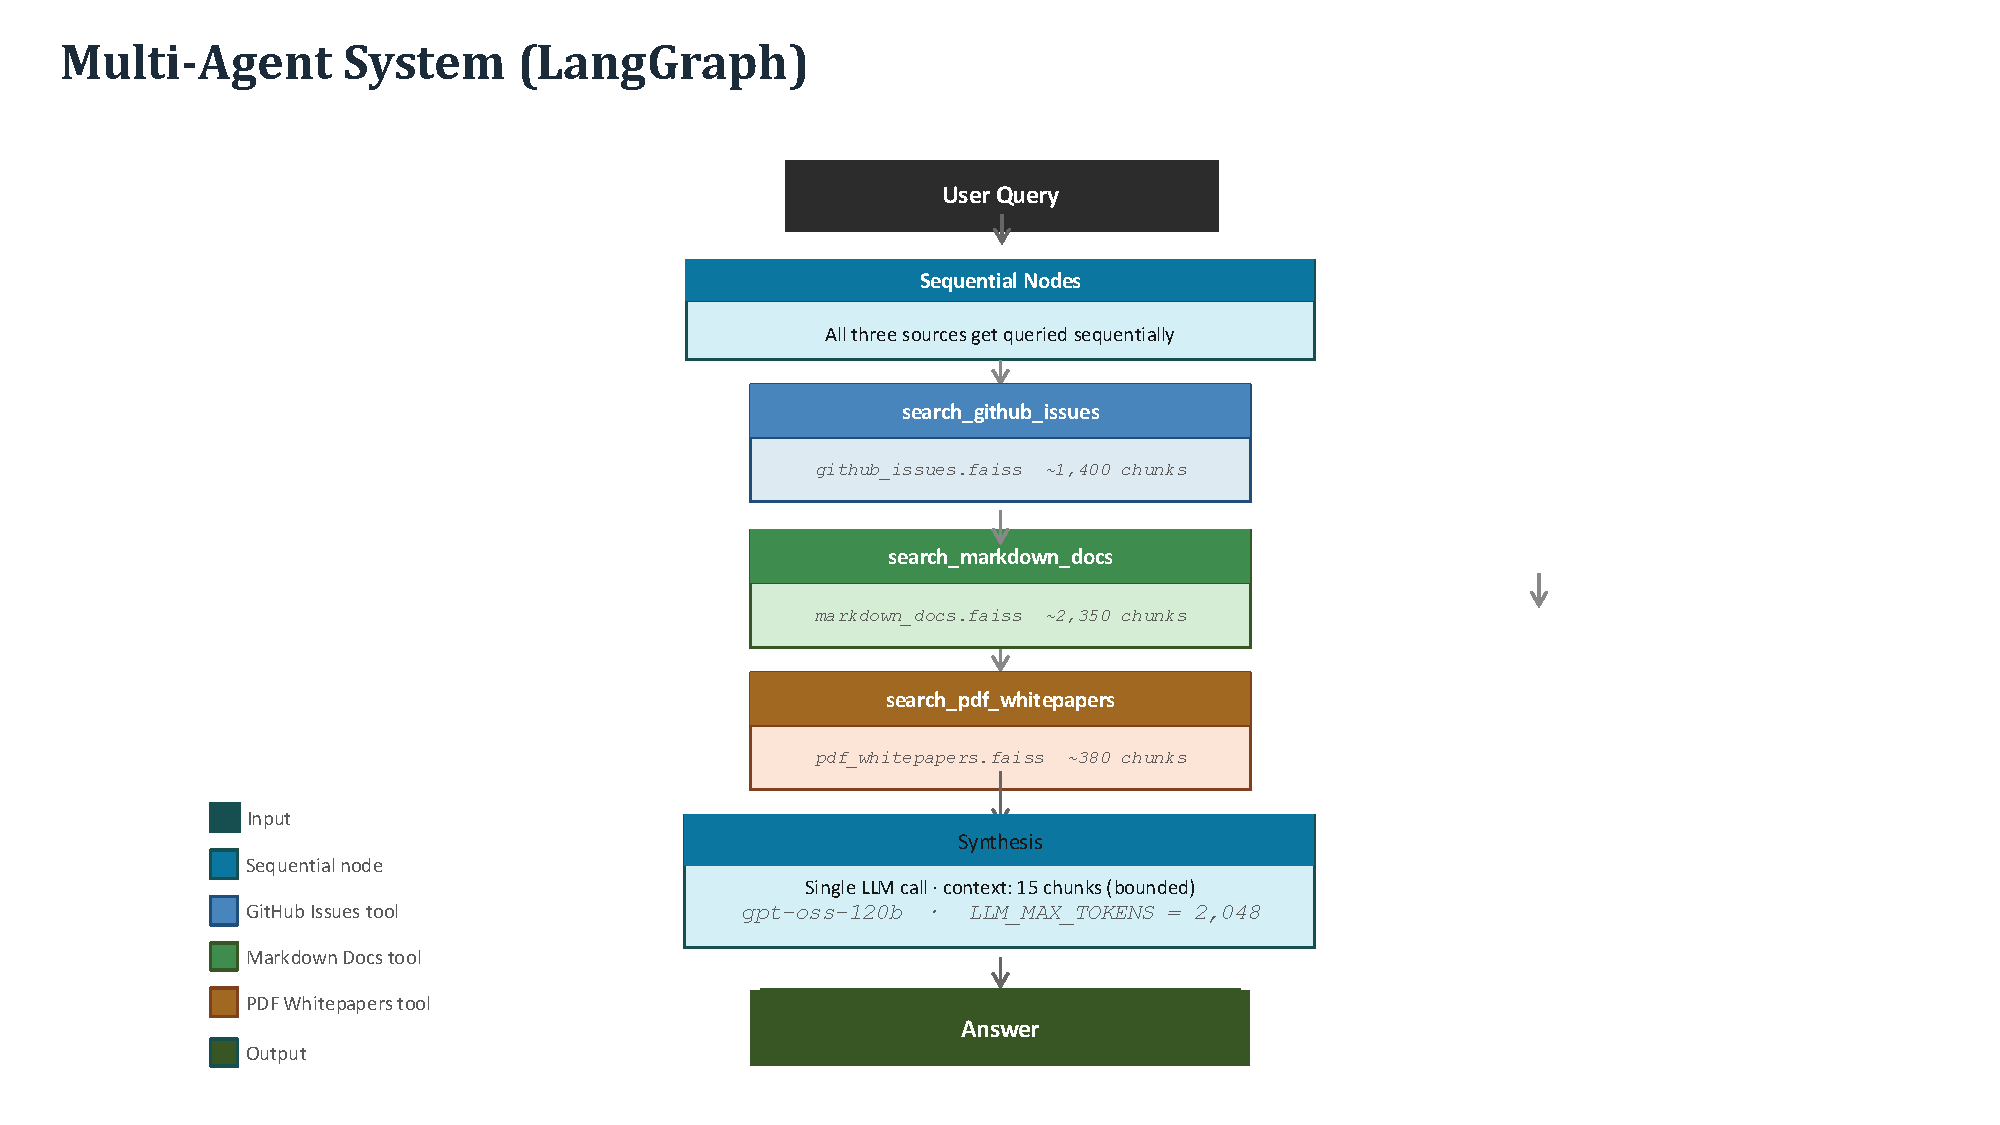
\includegraphics[width=\linewidth]{images/multi_agent}
  \caption{Multi-agent coordination architecture. A single \texttt{retrieve\_all\_sources} node queries all three per-source FAISS indexes sequentially, accumulating five chunks per source. The \texttt{synthesize} node then issues exactly one LLM call over the pooled fifteen-chunk context. There is no reasoning loop and no iteration limit.}
  \label{fig:multi_agent}
\end{figure}

\section{Comparability Design Decisions}

A valid architectural comparison requires that observed differences in evaluation outcomes be attributable to the retrieval and orchestration strategies under study rather than to differences in data, models, or hardware. Every component not itself under comparison is therefore held constant across both systems. Table~\ref{tab:comparability} lists the shared and varied parameters; the design decisions implicit in each row are elaborated below.

\subsection{Shared Experimental Parameters}

The language model, embedding model, chunking parameters, and reranker are identical across both systems. Both access the language model through the same OpenAI-compatible endpoint—Ollama locally, AI Refinery for evaluation—using the same model identifier and a generation temperature of zero. Temperature is fixed at zero to produce fully deterministic outputs; any repeated query to either system yields the same response, which is a prerequisite for reliable latency averaging and reproducible RAGAS scoring. Both systems embed queries and corpus chunks using \texttt{BAAI/bge-base-en-v1.5} with L2-normalised vectors and the same retrieval-prefix convention, and both apply \texttt{cross-encoder/ms-marco-MiniLM-L-6-v2} to a candidate pool of twenty, returning five chunks as the final retrieved context.

\begin{table}[ht]
\centering
\small
\setlength{\tabcolsep}{4pt}
\caption{Controlled and varied parameters across both systems.}
\label{tab:comparability}
\begin{tabular}{p{3.8cm}p{5.4cm}p{5.4cm}}
\hline
\textbf{Parameter} & \textbf{RAG Pipeline} & \textbf{Agent System} \\
\hline
Language model        & shared endpoint; swapped via \texttt{.env} & shared endpoint; swapped via \texttt{.env} \\
Embedding model       & BGE-base-en-v1.5 (768d)     & BGE-base-en-v1.5 (768d) \\
Chunking              & 400 words, 60-word overlap  & 400 words, 60-word overlap \\
Reranker              & MiniLM, top-5               & MiniLM, top-5 per tool call \\
Document corpus       & shared JSONL source files   & shared JSONL source files \\
Generation temperature & 0 (deterministic)          & 0 (deterministic) \\
Hardware and runtime  & local CPU, single venv      & local CPU, single venv \\
\hline
\textit{Index structure}  & Unified FAISS (4\,840 chunks) & Three per-source FAISS indexes \\
\textit{Query resolution} & Fixed 4-step pipeline         & Iterative loop, max 15 steps \\
\textit{Source routing}   & Implicit (unified index)      & Explicit (LLM tool selection) \\
\hline
\end{tabular}
\end{table}

The document corpus is shared at the source level: both systems read from the same three JSONL files in \texttt{data/corpus/}. Their index structures differ because the RAG pipeline consolidates all records into a single FAISS index while the agent builds three separate per-source indexes from the same files. The total chunk count differs marginally—4,840 in the unified index versus approximately 4,130 across the three agent indexes—because the Markdown corpus is lightly downsampled during agent ingestion to keep index sizes balanced. Both systems run in the same Python virtual environment on the same hardware, eliminating interpreter version, library dependency, and process-level differences as confounds in the latency measurements.

\subsection{Defining Equivalent Effort}

Implementation complexity is evaluated as a first-class metric in this thesis, corresponding to Research Question 3. To make this comparison defensible, complexity is operationalised through three observable proxies rather than through subjective judgements about code quality or design elegance.

Lines of non-blank, non-comment code are counted per component for four parallel components in each system: ingestion, retrieval or tools, generation or agent executor, and the pipeline orchestrator. Framework calls—including LangChain agent and tool definitions—count toward the agent's total, because they represent integration and configuration work a developer must write and maintain. The second proxy is the number of explicit configuration parameters in each system's \texttt{config.py} file, reflecting the number of decisions a practitioner must make to deploy or tune the system. The third proxy is the number of steps required to onboard a new data source: for the RAG pipeline this involves appending records to the unified ingestion script and re-running the embedding step; for the agent it additionally requires building a new per-source FAISS index, writing a new \texttt{@tool} function, and updating the tool descriptions in the system prompt. These three proxies together provide an objective basis for the rubric-based complexity scores presented in Chapter~\ref{ch:results}.
